% Рисунок из тетради: u = 1 на (0,1), продолженная нулём на (-1,2).
\begin{figure}[htbp]
\centering
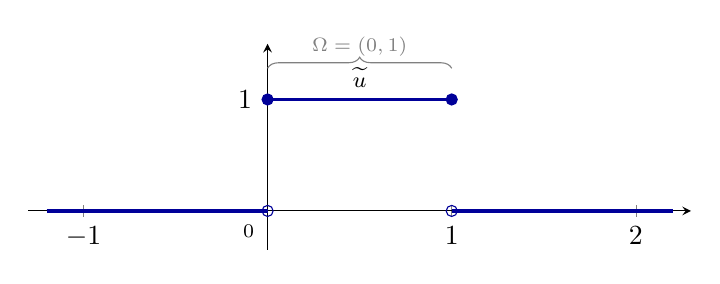
\begin{tikzpicture}
\begin{axis}[
  width=10cm, height=4.2cm,
  axis lines=middle,
  xmin=-1.3, xmax=2.3, ymin=-0.35, ymax=1.5,
  xtick={-1,1,2}, xticklabels={$-1$,$1$,$2$},
  ytick={1}, yticklabels={$1$},
  clip=false,
]
  \addplot[very thick, blue!60!black] coordinates {(-1.2,0) (0,0)};
  \addplot[very thick, blue!60!black] coordinates {(0,1) (1,1)};
  \addplot[very thick, blue!60!black] coordinates {(1,0) (2.2,0)};
  \addplot[only marks, mark=*, blue!60!black] coordinates {(0,1) (1,1)};
  \addplot[only marks, mark=o, blue!60!black] coordinates {(0,0) (1,0)};
  \node[anchor=south, font=\footnotesize] at (axis cs:0.5,1.02) {$\widetilde u$};
  \node[anchor=north east, font=\scriptsize] at (axis cs:-0.02,-0.04) {$0$};
  \draw[decorate, decoration={brace, amplitude=4pt}, gray]
    (axis cs:0,1.28) -- (axis cs:1,1.28);
  \node[gray, anchor=south, font=\scriptsize] at (axis cs:0.5,1.3) {$\Omega=(0,1)$};
\end{axis}
\end{tikzpicture}
\caption{Контрпример: $u \equiv 1$ на $\Omega=(0,1)$ лежит в $\Wp{p}{1}(\Omega)$,
но её продолжение нулём на $\widetilde\Omega = (-1,2)$ разрывно. Если бы
$u \in \Wpz{p}{1}(\Omega)$, продолжение лежало бы в $\Wp{p}{1}(\widetilde\Omega)$
и было бы абсолютно непрерывным, а значит непрерывным — противоречие.}
\label{fig:unit-ext}
\end{figure}
